\documentclass[tikz,12pt,border=2pt]{standalone}
\usepackage[T1]{fontenc}
\usepackage[scaled=0.92]{helvet}
\renewcommand{\familydefault}{\sfdefault}
\usetikzlibrary{calc}
\definecolor{accent}{RGB}{31,84,140}
\begin{document}
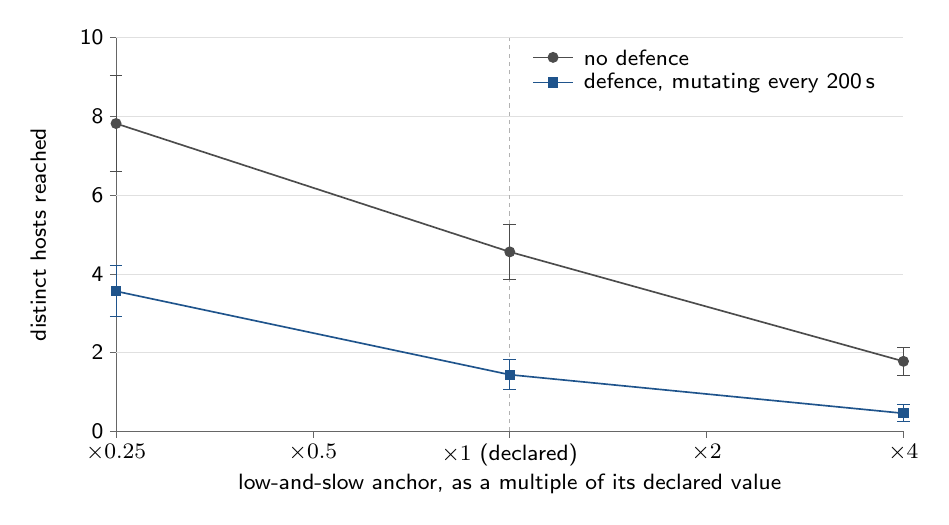
\begin{tikzpicture}[x=1cm,y=1cm,every node/.style={inner sep=1pt,font=\footnotesize}]
\draw[black!60,line width=0.4pt] (1.60,0.00) -- (11.60,0.00);
\draw[black!60,line width=0.4pt] (1.60,0.00) -- (1.60,5.00);
\draw[black!60,line width=0.3pt] (1.52,0.000) -- (1.60,0.000);
\node[anchor=east] at (1.48,0.000) {0};
\draw[black!60,line width=0.3pt] (1.52,1.000) -- (1.60,1.000);
\node[anchor=east] at (1.48,1.000) {2};
\draw[black!12,line width=0.2pt] (1.60,1.000) -- (11.60,1.000);
\draw[black!60,line width=0.3pt] (1.52,2.000) -- (1.60,2.000);
\node[anchor=east] at (1.48,2.000) {4};
\draw[black!12,line width=0.2pt] (1.60,2.000) -- (11.60,2.000);
\draw[black!60,line width=0.3pt] (1.52,3.000) -- (1.60,3.000);
\node[anchor=east] at (1.48,3.000) {6};
\draw[black!12,line width=0.2pt] (1.60,3.000) -- (11.60,3.000);
\draw[black!60,line width=0.3pt] (1.52,4.000) -- (1.60,4.000);
\node[anchor=east] at (1.48,4.000) {8};
\draw[black!12,line width=0.2pt] (1.60,4.000) -- (11.60,4.000);
\draw[black!60,line width=0.3pt] (1.52,5.000) -- (1.60,5.000);
\node[anchor=east] at (1.48,5.000) {10};
\draw[black!12,line width=0.2pt] (1.60,5.000) -- (11.60,5.000);
\node[rotate=90,anchor=south] at (0.75,2.50) {distinct hosts reached};
\draw[black!60,line width=0.3pt] (1.600,0.00) -- (1.600,-0.08);
\node[anchor=north] at (1.600,-0.12) {$\times0.25$};
\draw[black!60,line width=0.3pt] (4.100,0.00) -- (4.100,-0.08);
\node[anchor=north] at (4.100,-0.12) {$\times0.5$};
\draw[black!60,line width=0.3pt] (6.600,0.00) -- (6.600,-0.08);
\node[anchor=north] at (6.600,-0.12) {$\times1$ (declared)};
\draw[black!60,line width=0.3pt] (9.100,0.00) -- (9.100,-0.08);
\node[anchor=north] at (9.100,-0.12) {$\times2$};
\draw[black!60,line width=0.3pt] (11.600,0.00) -- (11.600,-0.08);
\node[anchor=north] at (11.600,-0.12) {$\times4$};
\draw[black!30,line width=0.3pt,dash pattern=on 1.5pt off 1.5pt] (6.600,0.00) -- (6.600,5.00);
\node[anchor=north] at (6.60,-0.50) {low-and-slow anchor, as a multiple of its declared value};
\draw[black!70,line width=0.4pt] (1.600,3.303) -- (1.600,4.517);
\draw[black!70,line width=0.4pt] (1.520,3.303) -- (1.680,3.303);
\draw[black!70,line width=0.4pt] (1.520,4.517) -- (1.680,4.517);
\draw[black!70,line width=0.4pt] (6.600,1.927) -- (6.600,2.633);
\draw[black!70,line width=0.4pt] (6.520,1.927) -- (6.680,1.927);
\draw[black!70,line width=0.4pt] (6.520,2.633) -- (6.680,2.633);
\draw[black!70,line width=0.4pt] (11.600,0.710) -- (11.600,1.070);
\draw[black!70,line width=0.4pt] (11.520,0.710) -- (11.680,0.710);
\draw[black!70,line width=0.4pt] (11.520,1.070) -- (11.680,1.070);
\draw[black!70,line width=0.6pt] (1.600,3.910) -- (6.600,2.280) -- (11.600,0.890);
\fill[black!70] (1.600,3.910) circle (0.7mm);
\fill[black!70] (6.600,2.280) circle (0.7mm);
\fill[black!70] (11.600,0.890) circle (0.7mm);
\draw[accent,line width=0.4pt] (1.600,1.454) -- (1.600,2.106);
\draw[accent,line width=0.4pt] (1.520,1.454) -- (1.680,1.454);
\draw[accent,line width=0.4pt] (1.520,2.106) -- (1.680,2.106);
\draw[accent,line width=0.4pt] (6.600,0.528) -- (6.600,0.912);
\draw[accent,line width=0.4pt] (6.520,0.528) -- (6.680,0.528);
\draw[accent,line width=0.4pt] (6.520,0.912) -- (6.680,0.912);
\draw[accent,line width=0.4pt] (11.600,0.121) -- (11.600,0.339);
\draw[accent,line width=0.4pt] (11.520,0.121) -- (11.680,0.121);
\draw[accent,line width=0.4pt] (11.520,0.339) -- (11.680,0.339);
\draw[accent,line width=0.6pt] (1.600,1.780) -- (6.600,0.720) -- (11.600,0.230);
\fill[accent] (1.600,1.780) ++(-0.65mm,-0.65mm) rectangle ++(1.3mm,1.3mm);
\fill[accent] (6.600,0.720) ++(-0.65mm,-0.65mm) rectangle ++(1.3mm,1.3mm);
\fill[accent] (11.600,0.230) ++(-0.65mm,-0.65mm) rectangle ++(1.3mm,1.3mm);
\draw[black!70,line width=0.6pt] (6.90,4.750) -- (7.40,4.750);
\fill[black!70] (7.15,4.750) circle (0.7mm);
\node[anchor=west] at (7.50,4.750) {no defence};
\draw[accent,line width=0.6pt] (6.90,4.430) -- (7.40,4.430);
\fill[accent] (7.15,4.430) ++(-0.65mm,-0.65mm) rectangle ++(1.3mm,1.3mm);
\node[anchor=west] at (7.50,4.430) {defence, mutating every 200\,s};
\end{tikzpicture}
\end{document}
